\documentclass{article}
\usepackage[utf8]{inputenc}
\usepackage[spanish]{babel}
\usepackage{amsmath}
\usepackage{amssymb}
\usepackage{amsfonts}
\usepackage{hyperref}
\usepackage{textcomp}
\usepackage{graphicx}
\usepackage{pgfplots}
\usepackage{geometry}
\usepackage{booktabs}
\hypersetup{
    colorlinks=true,
    linkcolor=black,
    citecolor=green,
    filecolor=magenta,      
    urlcolor=cyan,
}
\geometry{
  top=3cm,
  bottom=3cm,
  left=3cm,
  right=3cm
}

\title{Estadística 1}
\author{Jorge Miguel Alvarado Reyes}
\date{16 Agosto 2023}

\setlength{\parindent}{0pt}
\begin{document}

\begin{titlepage}
    \begin{center}
        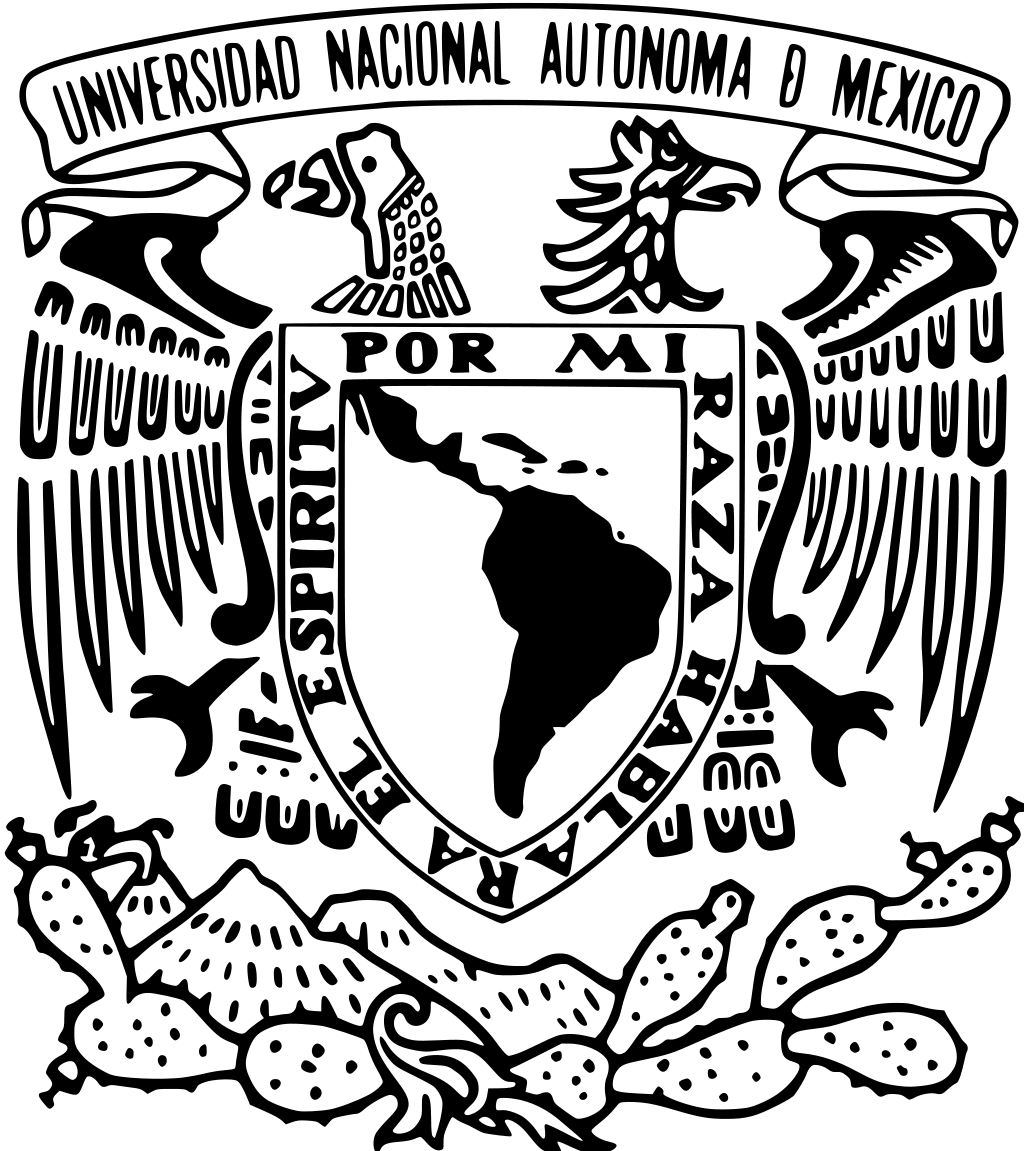
\includegraphics[width=0.2\textwidth]{../unam.png}
        \vspace*{.5cm}

        \LARGE
        \textbf{Universidad Nacional Autónoma de México}

        \vspace{0.5cm}
        \LARGE
        Facultad de Estudios Superiores Acatlán

        \vspace{2cm}

        \textbf{Apuntes} \\
        Estadística 2

        \vfill

        \vspace{1cm}

        \textbf{\large Autor:} \\
        Jorge Miguel Alvarado Reyes \\
        \vspace{.5cm}
        \normalsize \today

    \end{center}
\end{titlepage}
\newpage

\tableofcontents

\newpage

\section{29/01/2024}

\subsection{Objetivo general}

El estudiante aplicará pruebas no paramétricas, análisis de varianza, estadística bayesiana, análisis de regresión a la solución de problemas dentro de diversos campos de conocimiento.

\subsection{Temario}

\begin{enumerate}
    \item Pruebas no paramétricas
    \item Análisis de varianza y diseño de experimentos
    \item Análisis de regresión
    \item Inferencia bayesiana
\end{enumerate}

\subsection{Bibliografía}

\begin{itemize}
    \item Canavos, G. (1987). \textit{Probabilidad y estadística: Aplicación y métodos}.
    \item Lee, Peter M. (2012). \textit{Bayesian Statistics: An Introduction}.
    \item Montgomery, D. (2004) \textit{Diseño y análisis de experimentos}.
    \item \item Montgomery, D. (2002) \textit{Introducción al analisis de Regresion}.
\end{itemize}

\subsection{Evaluación}

\begin{itemize}
    \item Examenes parciales: 40\% (4 exámenes, uno por unidad)
    \item Prácticas: 30\%
    \item Tareas: 20\%
    \item Cuestionario: 10\% (Sobre el examen)
\end{itemize}

\subsection{Contacto}

\texttt{888745@pcpuma.acatlan.unam.mx}

\subsection{Examen diagnostico}
\begin{itemize}
    \item Medidas descriptivas
    \item Propiedades de los estimadores puntuales
    \item Intervalos de confianza
    \item Prueba de hipotesis
\end{itemize}

\section{02/02/2024}

\subsection{Solución del examen diagnóstico}

\textbf{Ejercicio 1}

Consideremos el conjunto $s = \{4, 2, 0, 9, 4, 2, -1, 1, -4, 2\}$.

A continuación, calculamos las medidas de tendencia central y de dispersión para el conjunto $s$:

\begin{itemize}
    \item \textbf{Media}: La media aritmética se calcula como el promedio de los valores del conjunto:
          \[
              \text{Media} = \frac{1}{n} \sum_{i=1}^{n}s_i
          \]
          donde $n$ es el número de elementos en el conjunto.

    \item \textbf{Moda}: La moda es el valor o valores que aparecen con mayor frecuencia en el conjunto. En caso de que todos los elementos aparezcan con la misma frecuencia, el conjunto se considera amodal.

    \item \textbf{Mediana}: La mediana es el valor que ocupa la posición central del conjunto una vez que este ha sido ordenado. Si el número de elementos es par, la mediana se calcula como el promedio de los dos valores centrales. Para nuestro conjunto ordenado, debemos calcularlo correctamente.

    \item \textbf{Varianza}: La varianza mide la dispersión de los valores del conjunto respecto a la media. Se calcula con la fórmula:
          \[
              \text{Varianza} = \frac{1}{n} \sum_{i=1}^{n}(s_i - \bar{x})^2
          \]
          donde $\bar{x}$ es la media del conjunto.

    \item \textbf{Rango}: El rango es la diferencia entre el valor máximo y el valor mínimo del conjunto. Se calcula como:
          \[
              \text{Rango} = X_{\text{max}} - X_{\text{min}}
          \]
\end{itemize}

\textbf{Ejercicio 2}

a)

\[\hat{\theta}_1 = \frac{3x_1 + 4x_4}{10} - \mu\]

\[\hat{\theta}_2 = \frac{5x_2 + 3x_3 +4x_4}{10}\]

\[\hat{\theta}_3 = \frac{x_1 + x_2 + x_3 + \sigma^2}{4}\]

\[\hat{\theta}_4 = \frac{2x_1 + 4x_2 + 4\mu + 2x_4}{12}\]

\[\hat{\theta}_5 = X_n\]

\[\hat{\theta}_6 = \Bar{X}\]

b)

Sesgo

\[\beta(\hat{\theta}) = E(\hat{\theta}) - \theta\]

\[- \beta(\hat{\theta}_2) = E(\hat{\theta}_2) - \mu\]

\[- \beta(\hat{\theta}_2) = E(\frac{5x_2 + 3x_3 + 4x_4}{10}) - \mu\]

\[\frac{1}{10} [5E(x_2) + 3E(x_3) + 4E(x_4)] - \mu\]

\[\frac{5\mu + 3 \mu + 4\mu}{10} - \mu\]

\[1.2\mu - \mu = 0.2\mu\]

\[- \beta(\hat{\theta}_5) = E(X_n) - \mu\]

\[- \beta(\hat{\theta}_5) = \mu - \mu = 0\]

\[- \beta(\hat{\theta}_6) = E(\bar{X}) - \mu\]

\[- \beta(\hat{\theta}_6) = \mu - \mu = 0\]

\textbf{Ejercicio 3}

Pruebas $t$: $X_1, \dots, X_n \sim N(\mu, \sigma^2), \mu = ?, \sigma^2 = ?$

Pruebas basadas en la distribución normal: $X_1, \dots, X_n \sim N(\mu, \sigma^2), \mu = ?$

Estandarizar una variable: $\frac{X - E(x)}{\sqrt{Var(x)}}$

En el ejercicio tenemo:

$X_1, \dots, X_n \sim N(\mu, \sigma^2), \mu = ?, \sigma = 30$

Intervalo de confianza:
\[\bar{X} \pm z_{\frac{\alpha}{z}} \sqrt{Var(\hat{\mu})}\]

\[\bar{X} \pm z_{\frac{\alpha}{z}} \frac{\sigma}{\sqrt{n}}\]

\[1550 \pm 1.96 \left(\frac{30}{\sqrt{50}}\right) = (1541.684, 1558.316)\]

Ejercicio 4:

\[X_1 \sim N(\mu, \sigma^2 = 1)\]

\[H_0: \mu = 0 vs H_1: \mu = 2\]

Región  de rechazo $ = \{x | x_1 \geq 1.5\}$

\[X_1 = 2 \geq 1.5 \rightarrow X_1 \sim N(2,1)\]

Probabilida del cometer el error 1:
Error 1 = Rachazar $H_0$ cuando es cierta
\[P(X_1 \geq 1.5 | \mu = 0) = 0.0668072\]

Probabilida del cometer el error 2:
Error 2 = No rechazar $H_0$ cuando es falsa
\[P(X_1 < 1.5 | \mu = 2) = 0.3085375\]

c) 1 - beta = 0.6914625

\section{07/02/2024}

\subsection{Unidad 1: Pruebas no parametricas}

\subsubsection{Introducción}

En este tipo de pruebas no se tiene el supuesto de que la muestra pertenece a una familia parametrica, como es el caso de las pruebas $F$ y $T$ que requieren que los datos se distribuyan como una normal. \\
En el caso parametrico se tiene que $X^{-} \sim f_x(x|\theta)$ deonde $f_x(x|\theta)$ es una función de distribución conocida y $\theta$ es desconocida.\\
Mientras que, en el caso no parametrico $X^{-} \sim f_x(\cdot)$ con $f_x(\cdot) \exists \mathbb{F}$ es el conjunto de todas las sfunciones de distribución

\subsubsection{Pruebas de bondad de ajuste}

Consisten en comparar las observaciones de una muestra aleatoria con aquellas que se esperan observar si la hipotesis nula es correcta.\\
El objetivo de las pruebas de bondad de ajuste es encontrar las hipótesis, $H_0: F = F_0$ contra $H_1: F \neq F_0$, donde $F_0$ es una distribución completa o parcialmente conocida.

\textbf{Prueba Ji-Cuadrada}

Se utiliza para variables discretas que tienen un número finito de categorías y se puede adaptar a variables continuas pero no es recomendable.\\
Es etsta prueba se comparan las frecuencias observadas en cada categoría respecto a las frecuencias esperadas bajo el supuesto de la hipótesis nula

\textbf{Estadistico de la prueba}

\[X^2 = \sum_{i=1}^{k} \frac{(N_i - np_i)^2}{np_i} \sim X^2_{(k-1)}\]

donde $N_i$ es la frecuencia observada en la i-ésima categoría y $np_i$ es la frecuencia esperada bajo $H_0$, ademas n es el tamaño de la muestra y k es el total de categorias.\\
Se rechaza $H_0$ con un nivel de significancia $\alpha$, si el Estadístico $x^2 > q_{X^2_{(k-1)}}^{(1-\alpha)}$ es decir.

\[R = \{\sum_{i=1}^{k} \frac{(N_i - np_i)^2}{np_i} > q_{X^2_{(k-1)}}^{(1-\alpha)}\}\]

p-valor = $\mathbb{P}(X^2_{(k-1)} > \sum_{i=1}^{k} \frac{(N_i - np_i)^2}{np_i})$

si p-valor $< \alpha$ entonces se rechaza $H_0$

\textbf{Interpretación del p-valor}

El nivel mínimo de probabilidad de obtener los valores observados o más extremos si la hipótesis nula es correcta.\\
Es el nivel de significancia más pequeno para el que la muestra obtenida obligada a rechazar la hipótesis nula.
\newpage
\section{12/02/2024}
\subsection{Función de Distribución Empírica}

La función de distribución empírica es una herramienta esencial en estadística para estimar la distribución de probabilidad de un conjunto de datos. Se construye a partir de una muestra y ofrece una estimación de la función de distribución acumulativa (CDF, por sus siglas en inglés) de la población original. Esta función se emplea en diversas áreas como el análisis exploratorio de datos, pruebas de hipótesis y el ajuste de distribuciones teóricas a conjuntos de datos empíricos.

La definición matemática de la función de distribución empírica, dada una muestra ordenada \(x_1, x_2, \ldots, x_n\), es:

\begin{equation}
    F_n(x) = \frac{1}{n} \sum_{i=1}^n I(x_i \leq x)
\end{equation}

donde:
\begin{itemize}
    \item \(F_n(x)\) representa la función de distribución empírica evaluada en \(x\),
    \item \(n\) es el tamaño de la muestra,
    \item \(I(x_i \leq x)\) es una función indicadora que adopta el valor de 1 si \(x_i \leq x\) y 0 en caso contrario.
\end{itemize}

Esta función es escalonada, incrementándose en \(1/n\) en cada uno de los datos \(x_i\) de la muestra. La función \(F_n(x)\) refleja la proporción de observaciones en la muestra que no superan el valor \(x\).

Propiedades destacadas de la función de distribución empírica incluyen:
\begin{enumerate}
    \item \textbf{No decreciente:} \(F_n(x)\) es una función que solo puede mantenerse constante o incrementar.
    \item \textbf{Límites:} \(F_n(x) = 0\) para todo \(x\) menor que el mínimo de la muestra, y \(F_n(x) = 1\) para \(x\) superior al máximo de la muestra.
    \item \textbf{Convergencia:} Bajo ciertas condiciones, \(F_n(x)\) converge hacia la verdadera CDF de la población, \(F(x)\), a medida que el tamaño de muestra \(n\) se incrementa indefinidamente. Este comportamiento se deriva del teorema del límite central, entre otros resultados fundamentales en teoría de la probabilidad.
\end{enumerate}

La construcción y visualización de la función de distribución empírica son sencillas, facilitando el análisis descriptivo y comparativo de distribuciones de datos. Además, su utilidad se extiende a métodos no paramétricos, como la prueba de Kolmogorov-Smirnov, que compara la distribución empírica de una muestra con una distribución teórica o con la de otra muestra.
\subsection{Estadístico de la Prueba en la Prueba de Kolmogorov-Smirnov}

El estadístico de la prueba de Kolmogorov-Smirnov (K-S) se emplea para comparar una distribución empírica con una distribución teórica, o dos distribuciones empíricas entre sí. Este cuantifica la máxima discrepancia entre las funciones de distribución acumulativa (CDF) implicadas. Existen dos variantes de la prueba K-S: unidireccional, que compara una muestra con una distribución teórica, y bidireccional, que compara dos muestras.

\textbf{Prueba K-S Unidireccional}

En la variante unidireccional, el estadístico de la prueba \(D\) se define como:

\begin{equation}
    D_n = \sup_x |F_n(x) - F(x)|
\end{equation}

donde:
\begin{itemize}
    \item \(D_n\) es el estadístico de la prueba.
    \item \(\sup_x\) representa el supremo (máximo absoluto) sobre todos los valores de \(x\).
    \item \(F_n(x)\) es la función de distribución empírica de la muestra.
    \item \(F(x)\) es la CDF teórica para comparación.
\end{itemize}

\textbf{Prueba K-S Bidireccional}

Para la comparación bidireccional de dos muestras empíricas, el estadístico se calcula como:

\begin{equation}
    D_{n,m} = \sup_x |F_{n}(x) - G_{m}(x)|
\end{equation}

donde:
\begin{itemize}
    \item \(D_{n,m}\) es el estadístico de la prueba.
    \item \(F_{n}(x)\) y \(G_{m}(x)\) son las funciones de distribución empíricas de las dos muestras, de tamaños \(n\) y \(m\), respectivamente.
\end{itemize}

\textbf{Interpretación}

El valor de \(D\) indica la mayor diferencia vertical entre las CDF comparadas. Un valor bajo sugiere que las distribuciones son similares, mientras que uno alto indica diferencias notables. La significancia estadística de \(D\) se evalúa comparándolo con un valor crítico de referencia, dependiendo del nivel de significancia \(\alpha\) y, en algunos casos, del tamaño de la muestra. Si \(D\) supera este valor crítico, se rechaza la hipótesis nula de igualdad de distribuciones. \\
\newpage
\textbf{Ejemplo 2}

Verifica que los siguientes datos se distribuyen como una normal estándar con un nivel de significancia de  0.01.

\[ [-1.26, -1.12, -0.99, -0.72, -0.15, 0.07 , 0.18, 0.29, 0.39, 0.45, 0.55, 0.59, 0.84, 0.86, 2.30, 2.57]
\]
\textbf{Paso 1: Entender la Hipótesis Nula y Alternativa}

Hipótesis Nula (H0): Los datos siguen la distribución teórica propuesta (normal estándar).

Hipótesis Alternativa (H1): Los datos no siguen la distribución teórica propuesta.

\textbf{Paso 2: Calcular el Estadístico de la Prueba}

\begin{table}[ht]
    \centering
    \caption{Verifica que los siguientes datos se distribuyen como una normal estándar con un nivel de significancia $\alpha=0.01$}
    \begin{tabular}{cccc}
        \toprule
        \( X \) & \( F_n(x) \) & \( F(x) \) & \( |F_n(x) - F(x)| \) \\
        \midrule
        -1.26   & 1/16         & 0.1038     & 0.0413                \\
        -1.12   & 2/16         & 0.1314     & 0.0064                \\
        -0.99   & 3/16         & 0.1611     & 0.0264                \\
        -0.72   & 4/16         & 0.2358     & 0.0142                \\
        -0.15   & 5/16         & 0.4404     & 0.1279                \\
        0.07    & 6/16         & 0.5279     & 0.1529                \\
        0.18    & 7/16         & 0.5714     & 0.1339                \\
        0.29    & 8/16         & 0.6141     & 0.1141                \\
        0.39    & 9/16         & 0.6517     & 0.0892                \\
        0.45    & 10/16        & 0.6736     & 0.0486                \\
        0.55    & 11/16        & 0.7088     & 0.0213                \\
        0.59    & 12/16        & 0.7224     & 0.0276                \\
        0.84    & 13/16        & 0.7995     & 0.0130                \\
        0.86    & 14/16        & 0.8051     & 0.0699                \\
        2.30    & 15/16        & 0.9893     & 0.0518                \\
        2.57    & 16/16        & 0.9949     & 0.0051                \\
        \bottomrule
    \end{tabular}
\end{table}

\begin{equation}
    D_{n,m} = \sup_x |F_{n}(x) - G_{m}(x)| = 0.1529
\end{equation}

\begin{equation}
    q_{n}(1-\alpha), n = 16, \alpha = 0.01 \\
\end{equation}
Buscar en la tabla el cuantil

\begin{equation}
    0.1529 <  q_{n}(1-\alpha)\\
\end{equation}

\begin{equation}
    0.1529 < 0.392
\end{equation}


Por lo tanto no se rechaza $H_0$ y $X \sim N(0,1)$

\newpage

\section{14/02/2024}

\subsection{Pruebas de Bondad de Ajuste}

Estas pruebas determinan si una muestra observada sigue una distribución específica. La elección de la prueba depende del tipo de variable:

\subsubsection{Para Variables Continuas}

\begin{itemize}
    \item \textbf{Prueba de Kolmogorov-Smirnov}
          \begin{itemize}
              \item \textit{Descripción}: Compara la distribución acumulativa de una muestra con una distribución teórica, evaluando la máxima diferencia.
              \item \textit{Supuestos}: Muestra independiente y aleatoria.
              \item \textit{Uso recomendado}: Comparar si la distribución de una muestra continua se ajusta a una distribución teórica específica.
          \end{itemize}
\end{itemize}

\subsubsection{Para Variables Discretas}

\begin{itemize}
    \item \textbf{Prueba de Ji-Cuadrada ($\chi^2$)}
          \begin{itemize}
              \item \textit{Descripción}: Evalúa la discrepancia entre las frecuencias observadas y las esperadas bajo una hipótesis nula.
              \item \textit{Supuestos}: Muestras grandes, expectativas de frecuencia en cada categoría mayores a 5.
              \item \textit{Uso recomendado}: Verificar ajuste en datos categóricos o independencia entre dos variables categóricas.
          \end{itemize}
\end{itemize}

\subsection{Pruebas Basadas en Rangos}

Alternativa no paramétrica para comparación de medianas cuando no se cumplen las suposiciones de normalidad.

\subsubsection{Para 2 Poblaciones}

\begin{itemize}
    \item \textbf{¿Son Independientes? Sí}
          \begin{itemize}
              \item \textit{Mann-Whitney U}
                    \begin{itemize}
                        \item \textit{Descripción}: Compara medianas de dos grupos independientes.
                        \item \textit{Supuestos}: Muestras independientes.
                        \item \textit{Uso recomendado}: Comparar tendencias centrales de dos muestras no relacionadas.
                    \end{itemize}
          \end{itemize}

    \item \textbf{¿Son Independientes? No}
          \begin{itemize}
              \item \textit{Wilcoxon de Rangos con Signos}
                    \begin{itemize}
                        \item \textit{Descripción}: Compara diferencias medias dentro de pares de observaciones relacionadas.
                        \item \textit{Supuestos}: Pares emparejados o medidas repetidas.
                        \item \textit{Uso recomendado}: Datos emparejados o medidas repetidas en el mismo grupo.
                    \end{itemize}
          \end{itemize}
\end{itemize}

\subsubsection{Para Más de 2 Poblaciones}

\begin{itemize}
    \item \textbf{¿Son Independientes? Sí}
          \begin{itemize}
              \item \textit{Kruskal-Wallis}
                    \begin{itemize}
                        \item \textit{Descripción}: Generalización de Mann-Whitney para más de dos grupos, comparando medianas.
                        \item \textit{Supuestos}: Muestras independientes entre sí.
                        \item \textit{Uso recomendado}: Comparar medianas de tres o más grupos independientes.
                    \end{itemize}
          \end{itemize}

    \item \textbf{¿Son Independientes? No}
          \begin{itemize}
              \item \textit{Friedman}
                    \begin{itemize}
                        \item \textit{Descripción}: Comparación de tres o más grupos relacionados, basada en rangos.
                        \item \textit{Supuestos}: Muestras relacionadas, como medidas repetidas.
                        \item \textit{Uso recomendado}: Para datos relacionados con tres o más condiciones o tratamientos.
                    \end{itemize}
          \end{itemize}
\end{itemize}

En las pruebas basadas en rango no se tiene que indicar la distribución de los datos, basta con que la distribución de la muestra sea continua

\subsubsection*{Definición (Rangos)}

Sea $x_1, x_2, \ldots, x_n$ una muestra aleatoria sin empates, es decir, $x_i \neq x_j$, $\forall i \neq j$. Se define el rango de $x_i$, denotado por $R(x_i)$, como la posición que ocupa esta observación cuando los datos se ordenan de menor a mayor.

\subsection{Prueba de Mann-Whitney}

Sea $x_1, x_2, \ldots, x_n \sim F_x$ y $y_1, y_2, \ldots, y_m \sim F_y$ dos muestras aleatorias independientes de dos poblaciones. La prueba de Mann-Whitney U contrasta las siguientes hipótesis en relación a las distribuciones, las medias esperadas y las medianas de las dos poblaciones:

\begin{itemize}
    \item Para las distribuciones:
          \begin{itemize}
              \item $H_0: F_x = F_y$ contra $H_1: F_x \neq F_y$
          \end{itemize}
    \item Para las medias esperadas:
          \begin{itemize}
              \item $H_0: E(x) = E(y)$ contra $H_1: E(x) \neq E(y)$
          \end{itemize}
    \item Para las medianas:
          \begin{itemize}
              \item $H_0: \text{Med}(x) = \text{Med}(y)$ contra $H_1: \text{Med}(x) \neq \text{Med}(y)$
          \end{itemize}
\end{itemize}
\textbf{Estadístico de la prueba}

El estadístico de la prueba Mann-Whitney $u$ se calcula como el menor de los dos valores $u_1$ y $u_2$, donde:

\[
    u_1 = nm + \frac{n(n+1)}{2} - T_1
\]
\[
    u_2 = nm + \frac{m(m+1)}{2} - T_2
\]

Donde $T_1$ y $T_2$ son las sumas de los rangos de las variables $X$ y $Y$, respectivamente.

\[
    u = \min(u_1, u_2)
\]

La esperanza matemática y la varianza del estadístico $u$ son:

\[
    E(u) = \frac{nm}{2}
\]
\[
    Var(u) = \frac{nm(n+m+1)}{12}
\]

Bajo la hipótesis nula, el estadístico normalizado $Z$ sigue una distribución normal estándar $N(0,1)$:

\[
    Z = \frac{u - E(u)}{\sqrt{Var(u)}}
\]

Se rechaza la hipótesis nula $H_0$ con un nivel de significancia $\alpha$, si el valor absoluto de $Z$ es mayor que el cuantil crítico $q_z(1-\frac{\alpha}{2})$ de la distribución normal estándar:

\[
    |Z| > q_z\left(1-\frac{\alpha}{2}\right)
\]

El $p$-valor se calcula como la probabilidad de obtener un valor tan extremo o más que el valor observado de $Z$ bajo la hipótesis nula:

\[
    p\text{-valor} = 2\mathbb{P}(Z > |z|)
\]

Si $p\text{-valor} < \alpha$, se rechaza $H_0$

\subsection*{Ejemplo 3}

Investigadores reunieron datos sobre el número de admisiones hospitalarias resultantes de choques de vehículos en diferentes días. A continuación, se presentan los resultados obtenidos para los viernes 6 y los viernes 13. Se utiliza un nivel de significancia de 0.05 para probar la aserción de que los viernes 13, el número de admisiones hospitalarias por choques de vehículos no se ve afectado.

\subsection*{Datos}

\textbf{Viernes 6:} 9, 6, 11, 11, 3, 5

\textbf{Viernes 13:} 13, 12, 14, 10, 4, 12

\subsection*{Hipótesis}

Las hipótesis a contrastar son:
\[
    H_0: F_x = F_y \quad \text{contra} \quad H_1: F_x \neq F_y
\]
\[
    H_0: E(x) = E(y) \quad \text{contra} \quad H_1: E(x) \neq E(y)
\]

\subsection*{Ordenación de los Datos y Cálculo de Rangos}

Al ordenar todos los datos de menor a mayor, obtenemos la siguiente secuencia:
\[
    \{3_1, 4_2, 5_3, 6_4, 9_5, 10_6, 11_7, 11_8, 12_9, 12_{10}, 13_{11}, 14_{12}\}
\]

Dado que tenemos 12 datos en total, es necesario ajustar los rangos para los valores que aparecen repetidos (empates). En este caso, los valores repetidos son 11 y 12.

Para los valores 11, que aparecen en las posiciones 7 y 8, el rango promedio sería $(7+8)/2 = 7.5$. Por lo tanto, el rango que corresponde a ambos 11 es 7.5.

Para los valores 12, que aparecen en las posiciones 9 y 10, el rango promedio sería $(9+10)/2 = 9.5$. Así, el rango que corresponde a ambos 12 es 9.5.

suma de los rangos de viernes 6
\[T_1 = 1 + 3 + 4 + 5 + 7.5 + 7.5 = 28\]

suma de los rangos de viernes 13
\[T_2 = 2 + 6 + 9.5 + 9.5 + 11 + 12 = 50\]

$n=6$
$m=6$

\textbf{Por que $n$ y $m$ son 6?}

En el contexto del análisis estadístico presentado, n y m representan los tamaños de las muestras de los dos grupos que se están comparando: las admisiones hospitalarias en viernes 6 y viernes 13, respectivamente. En este caso, ambos n y m son igual a 6 porque hay exactamente 6 datos (o observaciones) para cada uno de los dos grupos.

entonces

\[u_1 = nm + \frac{n(n+1)}{2} - T_1\]
\[u_1 = 6*6 + \frac{6(7+1)}{2} - 28 = 29\]

\[u_2\ = 7\]

\[u = min(u_1, u_2) = 7\]

\section{16/02/2024}

\textbf{Continuacion de la clase pasada}

\[E(u) = 18\]

\[Var(u) = 39\]

\[z = \frac{u - E(u)}{\sqrt{Var(u)}} = -1.76140\]

\[|z| = 1.76140\]

\[u = 7\]

\[q_z(1 - \frac{\alpha}{2}) = q_z(0.975) = 1.96\]

Se rechaza $H_0$ si

\[|z| > q_z(1-\frac{\alpha}{z})\]


\[H_0: F_x = F_y\]
\[H_1: F_x \neq F_y\]

p-valor $ = 2 \mathbb{P}(z > 1.76)$ \\
p-valor $ = 2 [1-\mathbb{P}(z < 1.76)]$ \\
p-valor $ = 2 [0.0392]$ \\
p-valor $ = 0.0392$

Se rechaza $H_0$ si

p-valor $ < \alpha$ \\
$0.0784 < 0.05$

\subsection{Prueba de Wilcoxon}

La prueba de Wilcoxon para muestras relacionadas es un test no paramétrico utilizado para comparar dos muestras relacionadas, emparejadas o medidas repetidas en un solo sujeto, con el objetivo de evaluar si sus distribuciones de población difieren.

\subsection*{Hipótesis}

Sea $X$ y $Y$ dos variables aleatorias representando dos tratamientos o condiciones con pares de observaciones dependientes $(X_1, Y_1),\dots ,(X_n, Y_n)$. Se desean contrastar las siguientes hipótesis:

\[
    H_0: F_x = F_y
\]
contra
\[
    H_1: F_x \neq F_y
\]

\subsection*{Estadístico de la Prueba}

El estadístico de la prueba, $T$, se define como el mínimo entre $T_{+}$ y $T_{-}$, donde:

\[
    T_{+} = \text{suma de los valores absolutos de los rangos positivos}
\]

\[
    T_{-} = \text{suma de los valores absolutos de los rangos negativos}
\]

Para cada par $(X_i, Y_i)$, calculamos la diferencia $D_i = X_i - Y_i$. Los rangos se asignan a los valores absolutos de estas diferencias, ignorando las diferencias que sean cero. $T_{+}$ es la suma de los rangos para las diferencias positivas, y $T_{-}$ es la suma de los rangos para las diferencias negativas.

\subsection*{Aproximación Normal}

Bajo la hipótesis nula y para un tamaño de muestra grande, el estadístico $T$ puede aproximarse por una distribución normal con las siguientes expectativas y varianza:

\[
    E(T) = \frac{n(n + 1)}{4}
\]

\[
    Var(T) = \frac{n(n + 1)(2n + 1)}{24}
\]

El valor $z$ se calcula entonces como:

\[
    z = \frac{T - E(T)}{\sqrt{Var(T)}}
\]

Este valor $z$ se compara con los valores críticos de la distribución normal estándar para determinar si se rechaza o no la hipótesis nula.


Se rechaza $H_0$ con un nivel de significancia$\alpha$, si

\[|z| > q_z(1-\frac{\alpha}{z})\]
o
\[\text{p-valor} = 2\mathbb{P}(z > |z|) < \alpha\]

\textbf{Ejemplo 4}

Los numeros de fusibles electricos defectuosos producidos por las lineas A y B se registraron a diario durante 10 dias, con los siguientes resultados:

\subsection*{Datos}
\begin{table}[ht]
    \centering
    \caption{Verifica que los siguientes datos se distribuyen como una normal estándar con un nivel de significancia $\alpha=0.05$}
    \begin{tabular}{ccccc}
        \toprule
        Linea A & Linea B & $| A - B|$ & Rango & R con signo \\
        \midrule
        170     & 201     & 31         & 10    & -10         \\
        164     & 179     & 15         & 7     & -7          \\
        140     & 159     & 19         & 8     & -8          \\
        184     & 195     & 11         & 5     & -5          \\
        174     & 177     & 3          & 1     & -1          \\
        142     & 170     & 28         & 9     & -9          \\
        191     & 183     & 8          & 2     & 2           \\
        169     & 179     & 10         & 4     & -4          \\
        161     & 170     & 9          & 3     & -3          \\
        200     & 212     & 12         & 6     & -6          \\
        \bottomrule
    \end{tabular}
\end{table}

El numero 2 positivo en la tabla es positivo porque la diferencia de $A - B$ de sus respectivas lineas es positiva

\[T_{+} = 2\]
\[T_{-} = 53\]

Estas T son la suma de los rangos

\[T = min(T_{+}, T_{-}) = 2\]

\[
    E(T) = \frac{n(n + 1)}{4} = \frac{10(10 + 1)}{4} = 27.5
\]

\[
    Var(T) = \frac{n(n + 1)(2n + 1)}{24} = 96.25
\]

\[
    z = \frac{T - E(T)}{\sqrt{Var(T)}} -2.5993
\]

\[\alpha = 0.05\]

\[q_z(1 - \frac{\alpha}{2}) = 1.96\]

Se rechaza $H_0$ si

\[|z| > q_z()\]

\[2.5993 > 1.96\]

Por lo tanto las funciones de densidad son diferentes

\section{19/02/2024}

\subsection{Prueba de Kruskal-Wallis}

Consideremos una característica $X$ presente en $k$ poblaciones independientes. Supongamos que estamos interesados en determinar si la distribución de $X$ es la misma en todas las $k$ poblaciones.

Sea $F_i$ la distribución de $X$ en la $i$-ésima población. Las hipótesis que se plantean son:

\begin{itemize}
    \item Hipótesis nula ($H_0$): Todas las distribuciones son iguales, es decir,
          \[ H_0: F_1 = F_2 = \cdots = F_k. \]
    \item Hipótesis alternativa ($H_1$): Al menos una de las distribuciones $F_i$ es diferente de las demás, es decir,
          \[ H_1: \text{Al menos una } F_i \text{ es diferente de las demás}. \]
\end{itemize}

\textbf{Estadístico de la prueba}

El estadístico de la prueba de Kruskal-Wallis, $H$, se calcula como:
\[ H = \frac{12}{n(n+1)} \sum_{i=1}^{k} \frac{R_i^2}{n_i} - 3(n+1) \sim X^2_{k-1}, \]
donde $n$ es el tamaño total de la muestra (la suma de los tamaños de todas las muestras), $n_i$ es el tamaño de la muestra para la $i$-ésima población, y $R_i$ es la suma de los rangos de las observaciones en la $i$-ésima muestra. Este estadístico sigue aproximadamente una distribución chi-cuadrado ($\chi^2$) con $k-1$ grados de libertad, bajo la hipótesis nula.


\textbf{Reglas de decisión}

Para tomar una decisión sobre la hipótesis nula $H_0$ con un nivel de significancia $\alpha$, se utilizan las siguientes reglas:

\begin{itemize}
    \item Se rechaza $H_0$ si el estadístico de la prueba $H$ es mayor que el valor crítico de la distribución chi-cuadrado con $k-1$ grados de libertad, es decir,
          \[ H > q_{\chi^2_{k-1}}(1- \alpha), \]
          donde $q_{\chi^2_{k-1}}(1- \alpha)$ es el cuantil $(1-\alpha)$-ésimo de la distribución chi-cuadrado con $k-1$ grados de libertad.

    \item Alternativamente, se rechaza $H_0$ si el p-valor asociado al estadístico de la prueba es menor que el nivel de significancia $\alpha$, es decir,
          \[ \text{p-valor} = \mathbb{P}(\chi^2_{k-1} > H) < \alpha. \]
\end{itemize}

Esto significa que si el estadístico de la prueba calculado $H$ es suficientemente grande o si el p-valor es suficientemente pequeño, tenemos evidencia estadística para rechazar la hipótesis nula de que todas las poblaciones tienen distribuciones idénticas.
\newpage
\subsection*{Ejemplo 5}

Se tomaron muestras aleatorias independientes de casas recientemente vendidas en 4 zonas residenciales de una ciudad. El objetivo es determinar si existen diferencias significativas entre las zonas con respecto al cociente entre el precio de venta y el valor catastral de las propiedades.

\subsection*{Datos}

Los datos son los siguientes:

% Tabla de Datos
\begin{table}[ht]
    \centering
    \caption{\textbf{Cocientes entre los precios de venta y el valor catastral}}
    \begin{tabular}{cccc}
        \toprule
        Zona 1 & Zona 2 & Zona 3 & Zona 4 \\
        \midrule
        1.19   & 1.08   & 0.98   & 1.12   \\
        1.05   & 1.23   & 1.19   & 1.14   \\
        1.14   & 1.26   & 1.08   & 1.31   \\
        1.25   & 1.10   & 0.93   & 1.12   \\
        1.29   & 1.18   & 1.23   & 1.19   \\
               & 1.14   & 1.18   &        \\
        \bottomrule
    \end{tabular}
\end{table}

\subsection*{Asignación de Rangos}

\begin{table}[ht]
    \centering
    \caption{Asigancion de rangos (Ordenamiento del menor al mayor asigandoles un numero)}
    \begin{tabular}{cccc}
        \toprule
        Zona 1      & Zona 2      & Zona 3      & Zona 4      \\
        \midrule
        $1.19_{16}$ & $1.08_{4}$  & $0.98_{2}$  & $1.12_{7}$  \\
        $1.05_{3}$  & $1.23_{18}$ & $1.19_{15}$ & $1.14_{11}$ \\
        $1.14_{9}$  & $1.26_{20}$ & $1.08_{5}$  & $1.31_{22}$ \\
        $1.25_{19}$ & $1.10_{6}$  & $0.93_{1}$  & $1.12_{8}$  \\
        $1.29_{21}$ & $1.18_{12}$ & $1.23_{17}$ & $1.19_{14}$ \\
                    & $1.14_{10}$ & $1.18_{13}$ &             \\
        \bottomrule
    \end{tabular}
\end{table}

\begin{itemize}
    \item 1.08 se repite en 4 y 5 $4+5/2 = 4.5$
    \item 1.12 se repite en 7 y 8 $7+8/2 = 7.5$
    \item 1.14 se repite en 9, 10 y 11, $9+10+11/3=10$
    \item 1.18 se repite en 12 y 13 $12 + 13 / 2 = 12.5$
    \item 1.19 se repite en 14 y 15 y 16 $14 + 15 + 16 / 2 = 15$
    \item 1.23 se repite en 17 y 18 $17 + 18 / 2 = 17.5$
\end{itemize}

Por lo tanto los rangos se asignaron de la siguiente manera:

% Tabla de Rangos Asignados
\begin{table}[ht]
    \centering
    \caption{\textbf{Asignación de rangos y su promedio en caso de repetición}}
    \begin{tabular}{cccc}
        \toprule
        Zona 1      & Zona 2        & Zona 3        & Zona 4       \\
        \midrule
        $1.19_{15}$ & $1.08_{4.5}$  & $0.98_{2}$    & $1.12_{7.5}$ \\
        $1.05_{3}$  & $1.23_{17.5}$ & $1.19_{15}$   & $1.14_{10}$  \\
        $1.14_{10}$ & $1.26_{20}$   & $1.08_{4.5}$  & $1.31_{22}$  \\
        $1.25_{19}$ & $1.10_{6}$    & $0.93_{1}$    & $1.12_{7.5}$ \\
        $1.29_{21}$ & $1.18_{12.5}$ & $1.23_{17.5}$ & $1.19_{15}$  \\
                    & $1.14_{10}$   & $1.18_{12.5}$ &              \\
        \bottomrule
    \end{tabular}
\end{table}

\subsection*{Cálculo de la Estadística de Prueba}

El número de observaciones ($n$) y la suma de rangos ($R$) para cada zona son:

% Tabla de n y Suma de Rangos
\begin{table}[ht]
    \centering
    \caption{\textbf{Número de observaciones y suma de rangos}}
    \begin{tabular}{cccc}
        \toprule
        Zona 1     & Zona 2       & Zona 3       & Zona 4     \\
        \midrule
        $n_1 = 5$  & $n_2 = 6$    & $n_3 = 5$    & $n_4 = 4$  \\
        $R_1 = 68$ & $R_2 = 70.5$ & $R_3 = 52.5$ & $R_4 = 62$ \\
        \bottomrule
    \end{tabular}
\end{table}

La estadística de prueba $H$ se calcula como:

\[ H = \frac{12}{n(n + 1)} \left(\sum \frac{R_i^2}{n_i}\right) - 3(N + 1) \]

Donde $N$ es el número total de observaciones. Para este caso:

\[ H = \frac{12}{22 \times 23} \left(\frac{68^2}{5} + \frac{70.5^2}{6} + \frac{52.5^2}{5} + \frac{62^2}{4}\right) - 3(22 + 1) = 1.70395 \]

\subsection*{Conclusión}

Se rechaza $H_0$ si
\[H > q_{X^{2}_{k-1}}(1 - \alpha)\]
\[1.70395 > q_{X^{2}_{k-1}}(0.95) = 7.815\]
No rechazamos $H_0$. Por lo tanto, concluimos que no hay evidencia suficiente para afirmar que existen diferencias significativas entre las zonas en cuanto al cociente entre el precio de venta y el valor catastral de las propiedades.

La expresión para el valor crítico de la distribución chi-cuadrado con 3 grados de libertad es:
\[X^2_3 = q_{X^2_3}(1-\alpha)\]

El cálculo del p-valor se realiza como sigue:
\[\text{p-valor} = \mathbb{P}(X^2_3 > 1.70395)\]

Para estimar el p-valor, se puede utilizar la aproximación a la distribución normal estándar, de manera que:
\[\mathbb{P}(X^2_3 > 1.70395) \approx \mathbb{P}\left(\frac{X - E(X)}{\sqrt{\text{Var}(X)}} > \frac{1.70395 - 3}{\sqrt{6}}\right)\]

Simplificando la expresión, obtenemos:
\[ = \mathbb{P}(Z > -0.53)\]

Finalmente, utilizando la tabla de la distribución normal estándar, calculamos el p-valor como:
\[= 1 - \mathbb{P}(Z < -0.53) = 1 - 0.2981 = 0.7019\]

\section{21/02/2024}

\subsection{Pruebas basadas en corridas}

Las pruebas basadas en corridas son utilizadas en estadística para determinar si una secuencia de elementos es aleatoria. Esto es particularmente útil para analizar patrones dentro de series de datos donde se espera una distribución aleatoria. Las hipótesis que se contrastan en este tipo de prueba son:

\begin{itemize}
    \item $H_0$: Los datos siguen una secuencia aleatoria.
    \item $H_1$: Los datos no siguen una secuencia aleatoria.
\end{itemize}

\subsubsection*{Estadística de la prueba}


La estadística de la prueba se basa en el número total de corridas ($R_t$), donde una \textit{corrida} se define como una secuencia ininterrumpida de elementos similares (por ejemplo, una serie de números crecientes o decrecientes).

\[R_t = \text{Número total de corridas}\]

\subsubsection*{Aproximación normal}

Bajo la hipótesis nula de aleatoriedad, el valor esperado y la varianza de $R_t$ pueden aproximarse mediante las siguientes fórmulas, donde $n_1$ y $n_2$ son el número de elementos en cada uno de los dos grupos definidos (por ejemplo, números por encima y por debajo de la mediana, presencia o ausencia de una característica):

\[\text{E}(R_t) = \frac{2n_1n_2}{n} + 1\]

\[\text{Var}(R_t) = \frac{2n_1n_2(2n_1n_2-n)}{n^2(n-1)}\]

Una vez calculados el valor esperado y la varianza, se puede utilizar la siguiente fórmula para determinar el valor \(z\), el cual indica cuántas desviaciones estándar se encuentra el número observado de corridas del esperado bajo la hipótesis nula:

\[z = \frac{R_t - \text{E}(R_t)}{\sqrt{\text{Var}(R_t)}}\]

Este valor de \(z\) se compara entonces con los valores críticos de la distribución normal estándar para determinar si se rechaza o no la hipótesis nula de aleatoriedad en los datos.

\subsection*{Ejemplo 6}


Consideremos la siguiente secuencia de datos para determinar si es aleatoria:

\[1, 0, 1, 0, 0, 0, 1, 1, 0, 1, 0, 1, 0, 1, 0\]

Para analizar la aleatoriedad, agrupamos los datos en corridas según su valor. Una \textit{corrida} se define como una secuencia consecutiva de números iguales. La secuencia se divide en los siguientes grupos (corridas):

\begin{itemize}
    \item Grupo 1: $1$
    \item Grupo 2: $0$
    \item Grupo 3: $0, 0, 0$
    \item Grupo 4: $1, 1$
    \item Grupo 5: $0$
    \item Grupo 6: $1$
    \item Grupo 7: $0$
    \item Grupo 8: $1$
    \item Grupo 9: $0$
    \item Grupo 10: $1$
    \item Grupo 11: $0$
\end{itemize}

Cada grupo representa una corrida, por lo que el número total de corridas (\(R_t\)) en esta secuencia es igual al número de grupos:

\[R_t = 11\]

Para calcular el valor esperado (\(E(R_t)\)) y la varianza (\(Var(R_t)\)) de las corridas bajo la hipótesis de aleatoriedad, primero identificamos \(n_1\) y \(n_2\), que son las cantidades de 1s y 0s respectivamente:

\[n_1 = 8 \quad \text{(número de 1s)}\]

\[n_2 = 7 \quad \text{(número de 0s)}\]

El total de observaciones (\(n\)) es la suma de \(n_1\) y \(n_2\):

\[n = n_1 + n_2 = 15\]

Con \(n_1\), \(n_2\), y \(n\) definidos, podemos proceder a calcular \(E(R_t)\) y \(Var(R_t)\) utilizando las fórmulas para la aproximación normal de la prueba de corridas, y luego determinar si la secuencia es aleatoria comparando el valor observado de \(R_t\) con el valor esperado bajo la hipótesis nula de aleatoriedad.

\newpage

\section{23/02/2024}

\subsection{Pruebas de Independencia}

\subsubsection*{Definición}

Una medida numérica de asociación para las variables aleatorias continuas $X$ y $Y$, denotada por $\mu_{x,y}$, es considerada una medida de dependencia si cumple con las siguientes propiedades:

\begin{enumerate}
    \item $0 \leq \mu_{x,y} \leq 1$, donde los límites inferior y superior representan la independencia total y la dependencia funcional perfecta, respectivamente.
    \item $\mu_{x,y} = \mu_{y,x}$, lo que indica que la medida de dependencia es simétrica respecto a $X$ y $Y$.
    \item $X$ y $Y$ son independientes si y solo si $\mu_{x,y} = 0$. Esto establece un criterio numérico para la independencia de $X$ y $Y$.
    \item $\mu_{x,y} = 1$ si y solo si $X$ y $Y$ son casi seguramente funciones estrictamente monótonas una de la otra. Esto describe una relación de dependencia funcional completa.
    \item Si $\alpha$ y $\beta$ son funciones estrictamente monótonas con probabilidad 1, entonces $\mu_{\alpha(x), \beta(y)} = \mu_{x,y}$. Esta propiedad asegura que la medida de dependencia es invariante bajo transformaciones monótonas.
    \item Si $\{X_n,Y_n\}$ es una secuencia de variables aleatorias continuas con cópulas subyacentes $C_n$ y si $\{C_n\}$ converge a una cópula $C$, entonces
          \[\lim_{n \to \infty} \mu_{C_n} = \mu_C.\]
          Esto establece la continuidad de la medida de dependencia en términos de convergencia de cópulas.
\end{enumerate}

Estas propiedades definen formalmente cómo se debe medir la dependencia entre dos variables aleatorias continuas y establecen criterios claros para su evaluación.

\subsection{Coeficiente de Correlación de Spearman}

El coeficiente de correlación de Spearman, denotado como $r_s$, es una medida no paramétrica de la correlación de rango, que evalúa la dependencia entre dos variables cuantificando la dirección y la intensidad de su asociación monótona.

La fórmula para calcular el coeficiente de Spearman es:

\[r_s = 1 - \frac{6 \sum_{i=1}^{n}d_i^2}{n(n^2 - 1)},\]

donde $d_i$ es la diferencia entre los rangos correspondientes de las dos variables, y $n$ es el número de observaciones.

\subsubsection*{Prueba del Coeficiente de Spearman}

Para evaluar la significancia estadística de la correlación de Spearman entre dos variables, se utiliza la siguiente prueba de hipótesis:

\begin{itemize}
    \item Hipótesis nula ($H_0$): No existe dependencia monótona entre las dos variables. Esto se formaliza como $F(x,y) = F(x)F(y)$, donde $F(x,y)$ es la distribución conjunta de las variables y $F(x)$, $F(y)$ son sus distribuciones marginales.
    \item Hipótesis alternativa ($H_1$): Existe una dependencia monótona entre las dos variables, lo que implica que $F(x,y) \neq F(x)F(y)$.
\end{itemize}

Para realizar el contraste se sigue el procedimiento:

\begin{enumerate}
    \item Ordenar los datos de cada variable y asignar rangos.
    \item Calcular las diferencias de rango $d_i$ para cada par de observaciones.
    \item Insertar los valores de $d_i$ en la fórmula de $r_s$ para obtener el coeficiente de Spearman.
    \item Utilizar el valor calculado de $r_s$ y el número de observaciones $n$ para determinar el valor $p$ asociado a través de tablas o software estadístico.
    \item Comparar el valor $p$ con un nivel de significancia preestablecido (usualmente 0.05 o 0.01) para decidir si se rechaza $H_0$.
\end{enumerate}

Este procedimiento permite evaluar si la correlación observada entre las variables es estadísticamente significativa, indicando la presencia de una relación monótona entre ellas.

\subsection*{Ejemplo 7}

Ocho profesores de ciencias han sido clasificados por un juez de acuerdo a su capacidad de enseñanza y todos han tomado la prueba. ¿Cuál es la correlación entre la calificación del juez y la calificación de la prueba?

\begin{table}[ht]
    \centering
    \caption{\textbf{Calificaciones y rangos de los profesores}}
    \begin{tabular}{cccccc}
        \toprule
        Profesor & Calf. Juez & Calf. Prueba & $R(x_i)$ & $R(y_i)$ & $d_i^2$ \\
        \midrule
        1        & 7          & 44           & 7        & 1        & 36      \\
        2        & 4          & 72           & 4        & 5        & 1       \\
        3        & 2          & 69           & 2        & 3        & 1       \\
        4        & 6          & 70           & 6        & 4        & 4       \\
        5        & 1          & 93           & 1        & 8        & 49      \\
        6        & 3          & 82           & 3        & 7        & 16      \\
        7        & 8          & 67           & 8        & 2        & 36      \\
        8        & 5          & 80           & 5        & 6        & 1       \\
        \bottomrule
    \end{tabular}
\end{table}

La diferencia de rangos (\(d_i\)) se calcula restando el rango de la calificación de la prueba (\(R(y_i)\)) del rango de la calificación del juez (\(R(x_i)\)) para cada profesor. Luego, elevamos al cuadrado esta diferencia para obtener \(d_i^2\), lo que nos ayuda a medir la discrepancia entre los rangos de las dos variables sin importar la dirección de la diferencia.

\[d_i^2 = (R(X_i) - R(Y_i))^2\]

Con la suma de $d_i^2$ igual a 144, calculamos la correlación de Spearman entre las calificaciones del juez y las calificaciones de la prueba utilizando la fórmula:


\[r_s = 1 - \frac{6 \sum_{i=1}^{n}d_i^2}{n(n^2 - 1)}\]

\[r_s = 1 - \frac{6 * 144}{8(8^2 - 1)}\]

donde $n$ es el número de observaciones (profesores), que en este caso es 8. La correlación de Spearman calculada es $-0.714$, lo que indica una fuerte correlación negativa entre las dos variables. Esto significa que a medida que una variable aumenta, la otra tiende a disminuir.

\section{26/02/2024}
\subsection*{Análisis de la Correlación de Spearman y Prueba de Hipótesis}

Una vez calculada la correlación de Spearman, es crucial determinar si esta correlación es estadísticamente significativa. Bajo la hipótesis nula \(H_0: \rho = 0\), no esperamos encontrar correlación entre las calificaciones del juez y las de la prueba. La correlación de Spearman, \(r_s\), debería ser 0 si \(H_0\) es cierta. Utilizamos la siguiente estadística de prueba que se distribuye aproximadamente como una normal estándar \(N(0,1)\) para muestras de tamaño considerable:

\[
    \frac{r_s - E(r_s)}{\sqrt{var(r_s)}}
\]

Donde \(E(r_s) = 0\) bajo \(H_0\), y \(var(r_s) = \frac{1}{n-1}\), siendo \(n\) el número de observaciones. Para nuestro caso, con \(n = 8\) y \(r_s = -0.714\), la estadística de prueba se calcula como:

\[
    \frac{-0.714 - 0}{\sqrt{\frac{1}{8-1}}} = -1.889
\]

Este resultado se compara con los valores críticos de la distribución \(N(0,1)\). Para un nivel de significancia \(\alpha = 0.05\) en una prueba de dos colas, los valores críticos son \(\pm 1.96\). Al no ser -1.889 menor que -1.96 ni mayor que 1.96, no rechazamos la hipótesis nula al nivel de significancia del 5\%. Esto indica que no hay evidencia suficiente para afirmar que existe una correlación significativa entre las dos variables evaluadas.

Para formalizar el proceso de toma de decisiones, se rechaza \(H_0\) si:

\[
    |z| > q_z(1-\frac{\alpha}{2})
\]

Utilizando el valor absoluto de \(z\), calculamos:

\[
    |z| = |\frac{r_s}{\sqrt{\frac{1}{n-1}}}| = |\sqrt{n-1}r_s|
\]

Sustituyendo los valores conocidos:

\[
    |z| = |\sqrt{8-1}-0.714| = |-1.889| \approx 1.889
\]

Comparando este valor con \(q_z(1-\frac{\alpha}{2}) = q_z(0.975)\), ($q_z(0.975)$ se calcula en phyton con \texttt{norm.ppf(1 - alpha / 2)}) aproximadamente 1.96, concluimos:

Dado que \(|z| = 1.889 > 1.96\) no se cumple, entonces no rechazamos la hipótesis nula \(H_0\) al nivel de significancia de \(0.05\). Por lo tanto, la calificación del juez y la calificación de la prueba son independientes

\subsection{Tau de Kendall}

La Tau de Kendall es una medida de correlación basada en el orden de los rangos de los datos, que evalúa la similitud entre las ordenaciones de los datos en dos variables. A diferencia de la correlación de Pearson, que evalúa la relación lineal entre variables cuantitativas, la Tau de Kendall se centra en la relación ordinal, lo que la hace útil en situaciones donde la relación no es necesariamente lineal.

\subsubsection*{Definición}

Consideremos un conjunto de observaciones de un vector aleatorio \((X, Y)\), donde \(X\) e \(Y\) son variables aleatorias continuas. Sea \((X_i, Y_i)\) y \((X_j, Y_j)\) dos observaciones distintas de este vector, con \(i \neq j\).

Definimos estas observaciones como \textbf{concordantes} si los pares se mueven en la misma dirección, es decir, si:
\[
    (x_i < x_j \text{ y } y_i < y_j) \quad \text{o} \quad (x_i > x_j \text{ y } y_i > y_j),
\]
lo que indica que tanto \(X\) como \(Y\) aumentan o disminuyen juntos.

Por otro lado, los pares se consideran \textbf{discordantes} si se mueven en direcciones opuestas, es decir, si:
\[
    (x_i < x_j \text{ y } y_i > y_j) \quad \text{o} \quad (x_i > x_j \text{ y } y_i < y_j),
\]
indicando que uno aumenta mientras el otro disminuye.

La Tau de Kendall, \(\tau\), se calcula como la diferencia entre la proporción de pares concordantes y la proporción de pares discordantes, sobre el total de pares. Esto proporciona una medida de la correlación entre las variables, donde un valor de \(\tau = 1\) indica una correlación perfecta, \(\tau = -1\) indica una correlación inversa perfecta, y \(\tau = 0\) sugiere que no hay correlación.

Si $(x_i - x_j)(y_i - y_j)$ son concordantes
\[(x_i - x_j)(y_i - y_j) \geq 0\]

Si $(x_i - x_j)(y_i - y_j)$ son discordantes
\[(x_i - x_j)(y_i - y_j) \leq 0\]

\subsubsection*{Cálculo de la Tau de Kendall}

Para calcular la Tau de Kendall, se siguen los siguientes pasos:

\begin{enumerate}
    \item Ordenar las observaciones de acuerdo con los valores de \(X\), manteniendo el emparejamiento con sus correspondientes valores de \(Y\).
    \item Para cada observación \((X_i, Y_i)\), contar el número de pares concordantes y discordantes comparándola con las demás observaciones \((X_j, Y_j)\) donde \(j > i\).
    \item Calcular \(\tau\) utilizando la fórmula:
          \[
              \tau = \frac{\text{Número de pares concordantes} - \text{Número de pares discordantes}}{\binom{n}{2}},
          \]
          donde \(\binom{n}{2}\) es el número total de combinaciones de pares únicas posibles entre las observaciones.
\end{enumerate}

La Tau de Kendall ofrece una medida robusta y fiable de la correlación ordinal, útil en análisis estadísticos donde las suposiciones de linealidad y normalidad no se cumplen, o cuando se trabaja con datos ordinales.
\newpage
\section{01/03/3034}

\subsection{Tablas de contingencia}

\textbf{1.5.3}

\subsubsection*{Version 1}
Dados los siguientes datos:

\begin{itemize}
    \item $r$: número de renglones
    \item $c$: número de columnas
\end{itemize}

Las hipótesis son:

\begin{itemize}
    \item $H_0$: $F(x,y) = F(x)F(y)$
    \item $H_1$: $F(x,y) \neq F(x)F(y)$
\end{itemize}

El estadístico de la prueba es:

\[ \chi^2 = \sum \left( \frac{(Fo - Fe)^2}{Fe} \right) \sim \chi^2_{(r-1)(c-1)} \]

Donde:

\begin{itemize}
    \item $Fo$: frecuencia observada
    \item $Fe$: frecuencia esperada
\end{itemize}

Se rechaza $H_0$ si:

\[ \chi^2 > \chi^2_{\alpha, (r-1)(c-1)} \]

Se rechaza $H_0$ si el p-valor \( \alpha \):

\[ p\text{-valor} = P(\chi^2_{(r-1)(c-1)} > \chi^2_{\text{estadístico}}) \]

\subsubsection*{Version 2}

ados dos eventos $X$ e $Y$, las hipótesis son:
\begin{itemize}
    \item $H_0$: $F(x,y) = F(x)F(y)$
    \item $H_1$: $F(x,y) \neq F(x)F(y)$
\end{itemize}

El estadístico de la prueba es:
\[ X^2 = \sum \frac{(Fo-FE)^2}{FE} \sim \chi^2_{(r-1)(c-1)} \]
donde:
\begin{itemize}
    \item $r$ es el número de renglones
    \item $c$ es el número de columnas
\end{itemize}

Se rechaza $H_0$ si:
\[ X^2 > \chi^2_{\alpha, (r-1)(c-1)} \]

Se rechaza $H_0$ si p-valor \( < \alpha \)
\[ \text{p-valor} = P(X^2_{(r-1)(c-1)} > \text{estadístico}) \]

\subsubsection{Ejemplo 9}

Un total de \( n=309 \) defectos en muebles fueron registrados y los defectos fueron clasificados en 4 tipos: A, B, C y D. Al mismo tiempo, cada pieza de mueble fue identificada por la línea de producción en la que se elaboró. Verifica que los defectos son independientes de la línea de producción.

\subsubsection*{Version Mike}
Frecuencias observadas: $F_0$
\begin{center}
    \begin{tabular}{c c c c | c}
        Tipos & 1  & 2  & 3   & suma \\
        \hline
        A     & 15 & 26 & 33  & 74   \\
        B     & 21 & 31 & 17  & 69   \\
        C     & 45 & 34 & 49  & 128  \\
        D     & 13 & 5  & 20  & 38   \\
        \hline
        Suma  & 94 & 96 & 119 & 309
    \end{tabular}
\end{center}

Frecuencias esperadas: $F_E$
\begin{center}
    \begin{tabular}{c c c c | c}
        Tipos & 1                     & 2                     & 3   & suma \\
        \hline
        A     & $\frac{94(74)}{309}$  & $\frac{96(74)}{309}$  & ... & 74   \\
        B     & $\frac{94(69)}{309}$  & $\frac{96(69)}{309}$  & ... & 69   \\
        C     & $\frac{94(128)}{309}$ & $\frac{96(128)}{309}$ & ... & 128  \\
        D     & $\frac{94(38)}{309}$  & $\frac{96(38)}{309}$  & ... & 38   \\
        \hline
        Suma  & 94                    & 96                    & 119
    \end{tabular}
\end{center}

Frecuencias esperadas: $F_E$
\begin{center}
    \begin{tabular}{c c c c }
        Tipos & 1     & 2     & 3     \\
        \hline
        A     & 22.51 & 22.99 & 28.49 \\
        B     & 20.99 & 21.43 & 26.57 \\
        C     & 38.94 & 39.76 & 49.29 \\
        D     & 11.56 & 11.80 & 14.63 \\
    \end{tabular}
\end{center}

\begin{equation}
    X^2 = \frac{(15-22.51)^2}{22.51} + \frac{(26-22.99)^2}{22.99} + \dots + \frac{(20-14.63)^2}{14.63}
\end{equation}

\begin{equation}
    X^2 = 2.50 + 0.39 + 0.71 + ... = 19.19
\end{equation}


\[
    q_{(X^2)_{(r-1)(c-1)}^{1-\alpha}} = q_{(X^2_6)^(0.95)} = 12.59
\]

Se rechaza $H_0$ si

\[X^2 > q_{(X^2_6)^0.95}\]

\[19.19 > 12.59\]

Se rechaza $H_0$, Por lo tanto, los tipos de defectos dependen de las líneas de producción.

El p-valor se calcula como sigue:

\begin{align*}
    \text{p-valor} & = P\left(\chi^2 > 19.19\right)                                                                                             \\
                   & = P\left(\frac{\chi^2 - E(\chi^2)}{\sqrt{\text{Var}(\chi^2)}} > \frac{19.19 - E(\chi^2)}{\sqrt{\text{Var}(\chi^2)}}\right) \\
                   & = P\left(Z > \frac{19.19 - 6}{\sqrt{12}}\right)                                                                            \\
                   & = P\left(Z > 3.81\right)                                                                                                   \\
                   & = 1 - P\left(Z \leq 3.81\right)                                                                                            \\
                   & = 1 - 0.9999 \approx 0
\end{align*}

Dado que el p-valor \( \leq \alpha = 0.05 \), entonces se acepta \( H_1 \).

\subsubsection*{Version ChatGPT}

\textbf{Enunciado}
Para ello, se observaron las siguientes frecuencias de defectos:

\begin{table}[h]
    \centering
    \begin{tabular}{l c c c c}
        \hline
        Tipo de Defecto & Línea 1 & Línea 2 & Línea 3 & Total \\
        \hline
        A               & 15      & 26      & 33      & 74    \\
        B               & 21      & 31      & 17      & 69    \\
        C               & 45      & 34      & 49      & 128   \\
        D               & 13      & 5       & 20      & 38    \\
        \hline
        Total           & 94      & 96      & 119     & 309   \\
        \hline
    \end{tabular}
    \caption{Frecuencias observadas (\( F_O \))}
\end{table}

Y se calcularon las frecuencias esperadas (\( F_E \)) bajo la hipótesis nula de independencia:

\begin{table}[h]
    \centering
    \begin{tabular}{l c c c c}
        \hline
        Tipo de Defecto & Línea 1                         & Línea 2                         & Línea 3      \\
        \hline
        A               & \( \frac{94 \times 74}{309} \)  & \( \frac{96 \times 74}{309} \)  & \( \ldots \) \\
        B               & \( \frac{94 \times 69}{309} \)  & \( \frac{96 \times 69}{309} \)  & \( \ldots \) \\
        C               & \( \frac{94 \times 128}{309} \) & \( \frac{96 \times 128}{309} \) & \( \ldots \) \\
        D               & \( \frac{94 \times 38}{309} \)  & \( \frac{96 \times 38}{309} \)  & \( \ldots \) \\
        \hline
    \end{tabular}
    \caption{Frecuencias esperadas (\( F_E \))}
\end{table}

Luego, se procedió a calcular el estadístico de prueba \( X^2 \):

\begin{equation}
    X^2 = \sum \frac{(F_0 - F_E)^2}{F_E} = \frac{(15-22.51)^2}{22.51} + \frac{(26-22.99)^2}{22.99} + \ldots + \frac{(20-14.63)^2}{14.63} = 19.19
\end{equation}

Se compara el valor calculado con el valor crítico del estadístico \( \chi^2 \) para el nivel de significancia deseado y los grados de libertad correspondientes (\( (r-1)(c-1) \)):

\[
    \chi^2_{\text{crítico}, 0.95, 6} = 12.59
\]

La hipótesis nula \( H_0 \), que postula la independencia, se rechazará si el estadístico de prueba es mayor que el valor crítico:

\[
    19.19 > 12.59
\]

Dado que esto se cumple, se concluye que hay suficiente evidencia para rechazar la hipótesis nula, indicando que los defectos no son independientes de la línea de producción

\subsection{Pruebas de una cola (Prueba de Mann-Whitney y Prueba de Wilcoxon)}

Las hipótesis para la Prueba de Mann-Whitney son:
\begin{align*}
    H_0 & : E(X) = E(Y) \quad \text{vs} \quad H_1: E(X) < E(Y)    \\
    H_0 & : E(X) \geq E(Y) \quad \text{vs} \quad H_1: E(X) < E(Y)
\end{align*}

Se rechaza \(H_0\) si:
\begin{equation*}
    \frac{T - E(T)}{\sqrt{\text{Var}(T)}} \leq z_{\alpha}
\end{equation*}

Para la Prueba Wilcoxon, las hipótesis son:
\begin{align*}
    H_0 & : E(X) = E(Y) \quad \text{vs} \quad H_1: E(X) > E(Y)    \\
    H_0 & : E(X) \leq E(Y) \quad \text{vs} \quad H_1: E(X) > E(Y)
\end{align*}

Se rechaza \(H_0\) si:
\begin{equation*}
    \frac{T - E(T)}{\sqrt{\text{Var}(T)}} \geq z_{\alpha}
\end{equation*}

En ambos casos, \( T \) es el estadístico de prueba y \( z_{\alpha} \) es el valor crítico de la distribución normal estándar para un nivel de significancia \( \alpha \).


\subsection{Pruebas que se deben usar en cada ejercicio de la tarea}

\begin{enumerate}
    \item Prueba de Mann-Whitney
    \item No menciono
    \item No menciono
    \item No menciono
    \item No menciono
    \item No menciono
    \item No menciono
    \item Ejercicio 8 (Pistas)\\
          $\tau_{x,y} = \frac{z(P-Q)}{n(n-1)} = \dots = 1 - \frac{4Q}{n(n-1)}$\\
          $p+a = \frac{n(n-1)}{2}$
    \item No menciono
    \item No menciono
\end{enumerate}

\subsubsection*{Fin Unidad 1}

\newpage

\section{11/03/2024}

\section*{Unidad 2 - Análisis de varianza y diseño de experimentos}

\subsection*{Introducción}

Un experimento es una prueba o una serie de pruebas en las que se hacen cambios deliberados en las variables de entrada de un sistema o un proceso para identificar las razones de los cambios que pueden registrarse en la respuesta de salida.

\vspace{.25cm}

El diseño de experimentos se refiere al proceso para planificar el experimento de tal forma que se recaben los datos adecuados que puedan analizarse con metodos estadisticos que llevaran a conclusiones validas y objetivas.

Los tres principios del diseño de experimentos son:

\begin{itemize}
    \item Realizacion de replicas
    \item Aleatorizacion
    \item Formacion de bloques
\end{itemize}

\subsection*{Lineamientos para diseñar experimentos}

\begin{itemize}
    \item Identificar el problema.
    \item Elección de factores, niveles y tratamientos.
    \item Definir la unidad experimental.
    \item Seleccionar las variables de respuesta.
    \item Elección del diseño experimental.
    \item Determinar el número de réplicas.
    \item Ejecutar el experimento.
    \item Analizar los datos.
    \item Conclusiones y recomendaciones.
\end{itemize}

\section{13/03/2024}

\subsection*{Factor controlable}
Es la característica que controlamos y cuyo efecto se desea estudiar.

\subsection*{Nivel}
Es la categoría estudiada del factor.

\subsection*{Tratamientos}
Combinaciones de los factores estudiados.

\subsection*{Unidad experimental}
Es la subdivisión del material que puede recibir un tratamiento de forma independiente.

\subsection*{Variable respuesta}
Es la característica que se va a medir en cada unidad experimental.

\subsection*{Diseño experimental}
Es la forma de asignar los tratamientos a las unidades experimentales.

\subsection*{Error experimental}
Describe la variación entre las unidades experimentales.

\subsection*{Ejemplo 1}
Supóngase que de un grupo se seleccionaron al azar 20 hombres y 20 mujeres. Después, estos grupos se dividen al azar en grupo experimental y grupo de control. Al grupo de control se le aplica una prueba después de desayunar; al grupo experimental se le aplica la misma prueba en ayuno. Identifica los factores, niveles, tratamientos de este experimento.

\subsection{Análisis de varianza}

El método de análisis de varianza consiste en probar si varias medidas poblacionales son iguales. Cuando las varianzas son iguales y desconocidas, de manera que las hipótesis que se contrastan son:

\[H_0: \mu_1 = \dots = \mu_k\]
\[H_1: \mu_i \neq \mu_j, \text{ para } i\neq j\]

para \(k\) poblaciones normales independientes y con varianza \(\sigma^2\).

\subsection{Diseño completamente aleatorizado}

Es un diseño completamente aleatorio, la asignación de los tratamientos a cada unidad experimental es de forma aleatoria. Además, todas las unidades experimentales son homogéneas.

\subsection{Modelo}

\[y_{ij} = \mu_i + E_{ij}\]

Donde \(y_{ij}\) es la variable respuesta del i-ésimo tratamiento y \(E_{ij}\) es el error experimental. En este caso, hay \(t\) tratamientos y \(r\) repeticiones.

\subsection{Modelo completo}

\[y_{ij} = \mu_i + E_{ij}\]

Cada tratamiento tiene una media diferente, es decir, el modelo completo es la representación de \(H_1\).

\subsection{Modelo reducido}

\[y_{ij} = \mu + E_{ij}\]

Cada tratamiento tiene la misma media, es decir, el modelo reducido es la representación de \(H_0\).

El ojetivo es estimar los parametros de ambos modelos y determinar cual de los dos se ajusta mas a los datos observados.

Para la solucionar este problema, se utilizaran los estimadores de minimos cuadrados que se obtienen al minimizar la suma de los cuadrados de los errores experimentales

Estimador del modelo completo

\[y_{ij} = \mu_{i} + E_{ij}\]
\[E_{ij} = y_{ij} - \mu_{i}\]

Por lo anterior, la suma de los cuaddrados de los errores del modelo completo es:

\[ SS_{Ec} = \sum_{t}^{i=1} \sum_{r}^{j=1} (y_{ij} - \mu_{i})^2\]

para una $i$ fija

\[
    \frac{d[\sum_{r}^{j=1}(y_{ij} - \mu_{i})^2]}{d\mu_i} = \frac{d [\sum_{r}^{j=1} (y^{2}_{ij} - 2y_{ij}\mu_{i} + \mu^2_{i})]}{d\mu_i} = \sum_{r}^{j=1}(-2y_{ij} + 2\mu_i)
\]

al igualar a cero se tiene que

\[-2(\sum_{r}^{j=1}) = 0\]

\[-2\sum_{r}^{j=1} - r \mu_i = 0\]

\[\mu_i = \frac{\sum_{r}^{j=1} y_{ij}}{r}\]

Estimador de modelo reducido

\[ y_{ij} = \mu + E_{ij}\]
\[E_{ij} = y_{ij} - \mu\]

Por lo tanto la suma de los cuadrados de los errores del modelo reducido es

\[
    SS_{E_r} = \sum_{t}^{i=1} \sum_{r}^{j=1}(y_{ij} - \mu)^2
\]

A continuacion, encontramos el punto critico de la funcion $SS_{E_r}$
\end{document}
